\documentclass[aspectratio=169,11pt]{beamer}
\usepackage{teaching_slides}


% \usepackage{slashbox}
\title[L12a - Maximum Likelihood]{ Econometrics I}
\subtitle{Lecture 12a: Maximum Likelihood}
\author{Chris Conlon \\NYU Stern}
\date{Fall 2026}

\newcommand{\fp}{\frame[plain]}


\begin{document}
\maketitle

\begin{frame}{Introduction}
Consider a linear regression with $\varepsilon_i \mid X_i \sim \mathcal{N}(0,\sigma^2)$
\begin{align*}
Y_{i} &= X_{i}\, \beta + \varepsilon_{i}
\end{align*}
We've discussed the \alert{least squares estimator}:
\begin{align*}
\widehat{\beta}_{ols} &= \arg \min_{\beta} \sum_{i=1}^N (Y_i - X_i \beta)^2\\
\widehat{\beta}_{ols} &= (\mathbf{X}'\mathbf{X})^{-1} \mathbf{X}' \mathbf{Y}
\end{align*}
\end{frame}


\begin{frame}{Review: What is a Likelihood?}
Suppose we write down the joint distribution of our data $(y_i,x_i)$ for $i=1,\ldots,n$.
\begin{align*}
\Pr(y_1,\ldots,y_n, x_1,\ldots,x_n \mid  \theta)
\end{align*}
If  $(y_i,x_i)$ are I.I.D then we can write this as:
\begin{align*}
 \Pr(y_1,\ldots,y_n, x_1,\ldots,x_n \mid \theta) = \prod_{i=1}^N \Pr(y_i, x_i \mid \theta) \propto \prod_{i=1}^N \Pr(y_i \mid x_i , \theta)=\mathbb{L}( \mathbf{y} \mid \mathbf{x} ,\theta )
\end{align*}
(the $\propto$ step requires that the distribution of $x_i$ does not depend on $\theta$).
We call this $\mathbb{L}( \mathbf{y}\mid \mathbf{x} ,\theta )$ the \alert{likelihood} of the observed data.
\end{frame}




\begin{frame}{MLE: Example}
If we know the distribution of $\varepsilon_i$ we can construct a \alert{maximum likelihood estimator}
\begin{align*}
(\widehat{\beta}_{MLE},\widehat{\sigma}^2_{MLE}) &= \arg \max_{\beta,\sigma^2} \mathbb{L}(\beta,\sigma^2)
\end{align*}
Where 
\begin{align*} 
\mathbb{L}(\beta,\sigma^2) &= \prod_{i=1}^N \Pr(y_i \mid x_i,\beta,\sigma^2) \\
                  &= \prod_{i=1}^N \frac{1}{\sqrt{2 \pi \sigma^2}} \exp \left[-\frac{1}{2\sigma^2}(Y_i - X_i \beta)^2 \right]\\
\ell(\beta,\sigma^2) &= -\frac{N}{2} \ln (2 \pi \sigma^2) - \frac{1}{2 \sigma^2} \sum_{i=1}^N(Y_i - X_i \beta)^2
\end{align*}
\end{frame}

\begin{frame}{MLE: FOC's}
Take the FOC's of: 
$\ell(\beta,\sigma^2) = -\frac{N}{2} \ln (2 \pi \sigma^2) - \frac{1}{2 \sigma^2} \sum_{i=1}^N(Y_i - X_i \beta)^2
$:
\begin{align*} 
\frac{ \partial \ell(\beta,\sigma^2) }{\partial \beta}&= \frac{1}{ \sigma^2}\sum_{i=1}^N X_i'(Y_i - X_i \beta) = 0 \rightarrow \widehat{\beta}_{MLE}= \widehat{\beta}_{OLS}\\ 
\frac{ \partial \ell(\beta,\sigma^2) }{\partial \sigma^2}&= -\frac{N}{2 \sigma^2}  +  \frac{1}{2 \sigma^4} \sum_{i=1}^N(Y_i - X_i \beta)^2 = 0 \\
\widehat{\sigma}^2_{MLE} &= \frac{1}{N} \sum_{i=1}^N (Y_i - X_i \widehat{\beta}_{MLE})^2
\end{align*}
Note: the unbiased estimator uses $\frac{1}{N-K}$ ($K$ parameters, including the intercept).
\end{frame}

\begin{frame}{MLE: General Case}
\begin{enumerate}
\item Start with the \alert{joint density of the data} $Z_1,\ldots,Z_N$ with density $f_Z(z,\theta)$
\item Construct the likelihood function of the sample $z_1,\ldots,z_n$
\begin{align*}
\mathbb{L}(\mathbf{z} \mid  \theta) = \prod_{i=1}^N f_Z(z_i,\theta)
\end{align*}
\item Construct the \alert{log likelihood} (this has the same $\arg \max$)
\begin{align*}
\ell(\mathbf{z} \mid \theta) = \sum_{i=1}^N \ln f_Z(z_i,\theta)
\end{align*}
\item Take the FOC's to find $\widehat{\theta}_{MLE}$ that solves
\begin{align*}
\frac{\partial \ell(\theta)}{\partial \theta} =0 \text{ or  } \nabla_{\theta} \ell(\theta) =0 \text{ or  } \sum_{i=1}^N \frac{\partial \ln f_Z(z_i,\theta) }{\partial \theta}  =0.
\end{align*}
\end{enumerate}
\end{frame}

\begin{frame}{MLE in Detail}
Basic Setup: we know the form of $F(z \mid \theta)$ but not $\theta_0$. We know $\theta_0 \in \Theta \subset \mathbb{R}^K$.
\begin{itemize}
\item Begin with a sample of $z_i$ from $i=1,\ldots,N$ which are I.I.D. with CDF $F(z|\theta_0)$.
\item The MLE chooses
\begin{align*}
\widehat{\theta}_{MLE} = \arg \max_{\theta} \ell(\theta) = \arg \max_{\theta} \sum_{i=1}^N \ln f_Z(z_i,\theta)
\end{align*}
\item In practice the computer typically \alert{minimizes negative log-likelihood} so that $\widehat{\theta}_{MLE} = \arg \min_{\theta} - \ell(\theta)$.
\end{itemize}
\end{frame}


\begin{frame}{MLE: Technical Details}
\begin{enumerate}
\item Consistency. When is it true that, for every $\varepsilon>0$,
\begin{align*}
\lim _ { N \rightarrow \infty } \Pr \left( \left\| \hat { \theta } _ { MLE } - \theta _ { 0 } \right\| > \varepsilon \right) = 0
\end{align*}
\item Asymptotic Normality. What else do we need to show?
\begin{align*}
\sqrt { N } \left( \hat { \theta } _ { MLE } - \theta _ { 0 } \right) \stackrel { d } { \longrightarrow } \mathcal { N } \left( 0 , - \E \left[  \frac { \partial ^ { 2 }\log f(Z _ { i } , \theta _ { 0 } ) } { \partial \theta \partial \theta ^ { \prime } }   \right] ^ { - 1 } \right)
\end{align*}
\item Optimization. How do we obtain $\widehat{\theta}_{MLE}$ anyway?
\end{enumerate}
\end{frame}


\begin{frame}{MLE: Example \# 1}
\begin{itemize}
\item $Z_i \sim \mathcal{N}(\theta_0,1)$ and $\Theta = (-\infty,\infty)$. In this case:
\begin{align*}
\ell ( \theta ) = - \frac{N}{2} \ln ( 2 \pi ) - \sum _ { i = 1 } ^ { N } \left( z _ { i } - \theta \right) ^ { 2 } / 2
\end{align*}
\item MLE is $\widehat{\theta}_{MLE}=\overline{z}$ which is consistent for $\theta_0 = \E[Z_i]$
\item Asymptotic distribution is $\sqrt{N} ( \overline{z}-\theta_0) \sim \mathcal{N}(0,1)$.
\item Calculating mean is easy!
\end{itemize}
\end{frame}




\begin{frame}{MLE: Example \# 2}
\begin{itemize}
\item $Z_i = (Y_i, X_i)$ where  $X_i$ has finite mean and variance (but arbitrary distribution)
\item $(Y_i | X_i  =x) \sim  \mathcal{N}(x' \beta_0, \sigma_0^2)$
\begin{align*}
\widehat{\beta}_{MLE} &= (X'X)^{-1} X'Y\\
\widehat{\sigma}^2_{MLE} &= \frac{1}{N} \sum (y_i - x_i \widehat{\beta}_{MLE})^2
\end{align*}
\item We already have shown consistency and AN for linear regression with normally distributed errors...
\end{itemize}
\end{frame}


\begin{frame}{MLE: Example \# 3}
\begin{itemize}
\item $Z_i = (Y_i, X_i)$ where  $X_i$ has finite mean and variance (but arbitrary distribution)
\item $\Pr(Y_i=1 | X_i =x) =  \frac{e^{x' \theta_0}}{1+ e^{x'\theta_0}}$
\item Solution is the \alert{logit} model.
\item No simple MLE solution, establishing properties is not obvious...
\end{itemize}
\end{frame}

\begin{frame}{Jensen's Inequality}
\begin{columns}[T]
\begin{column}{.4\textwidth}
Let $\phi(z)$ be a convex function.\\ 
\vspace{2cm}
Then $\E[\phi(Z)] \geq \phi(\E [Z])$, with strict inequality if $\phi$ is strictly convex and $Z$ is non-degenerate.
\end{column}
\hfill
\begin{column}{.6\textwidth}
\begin{center}
 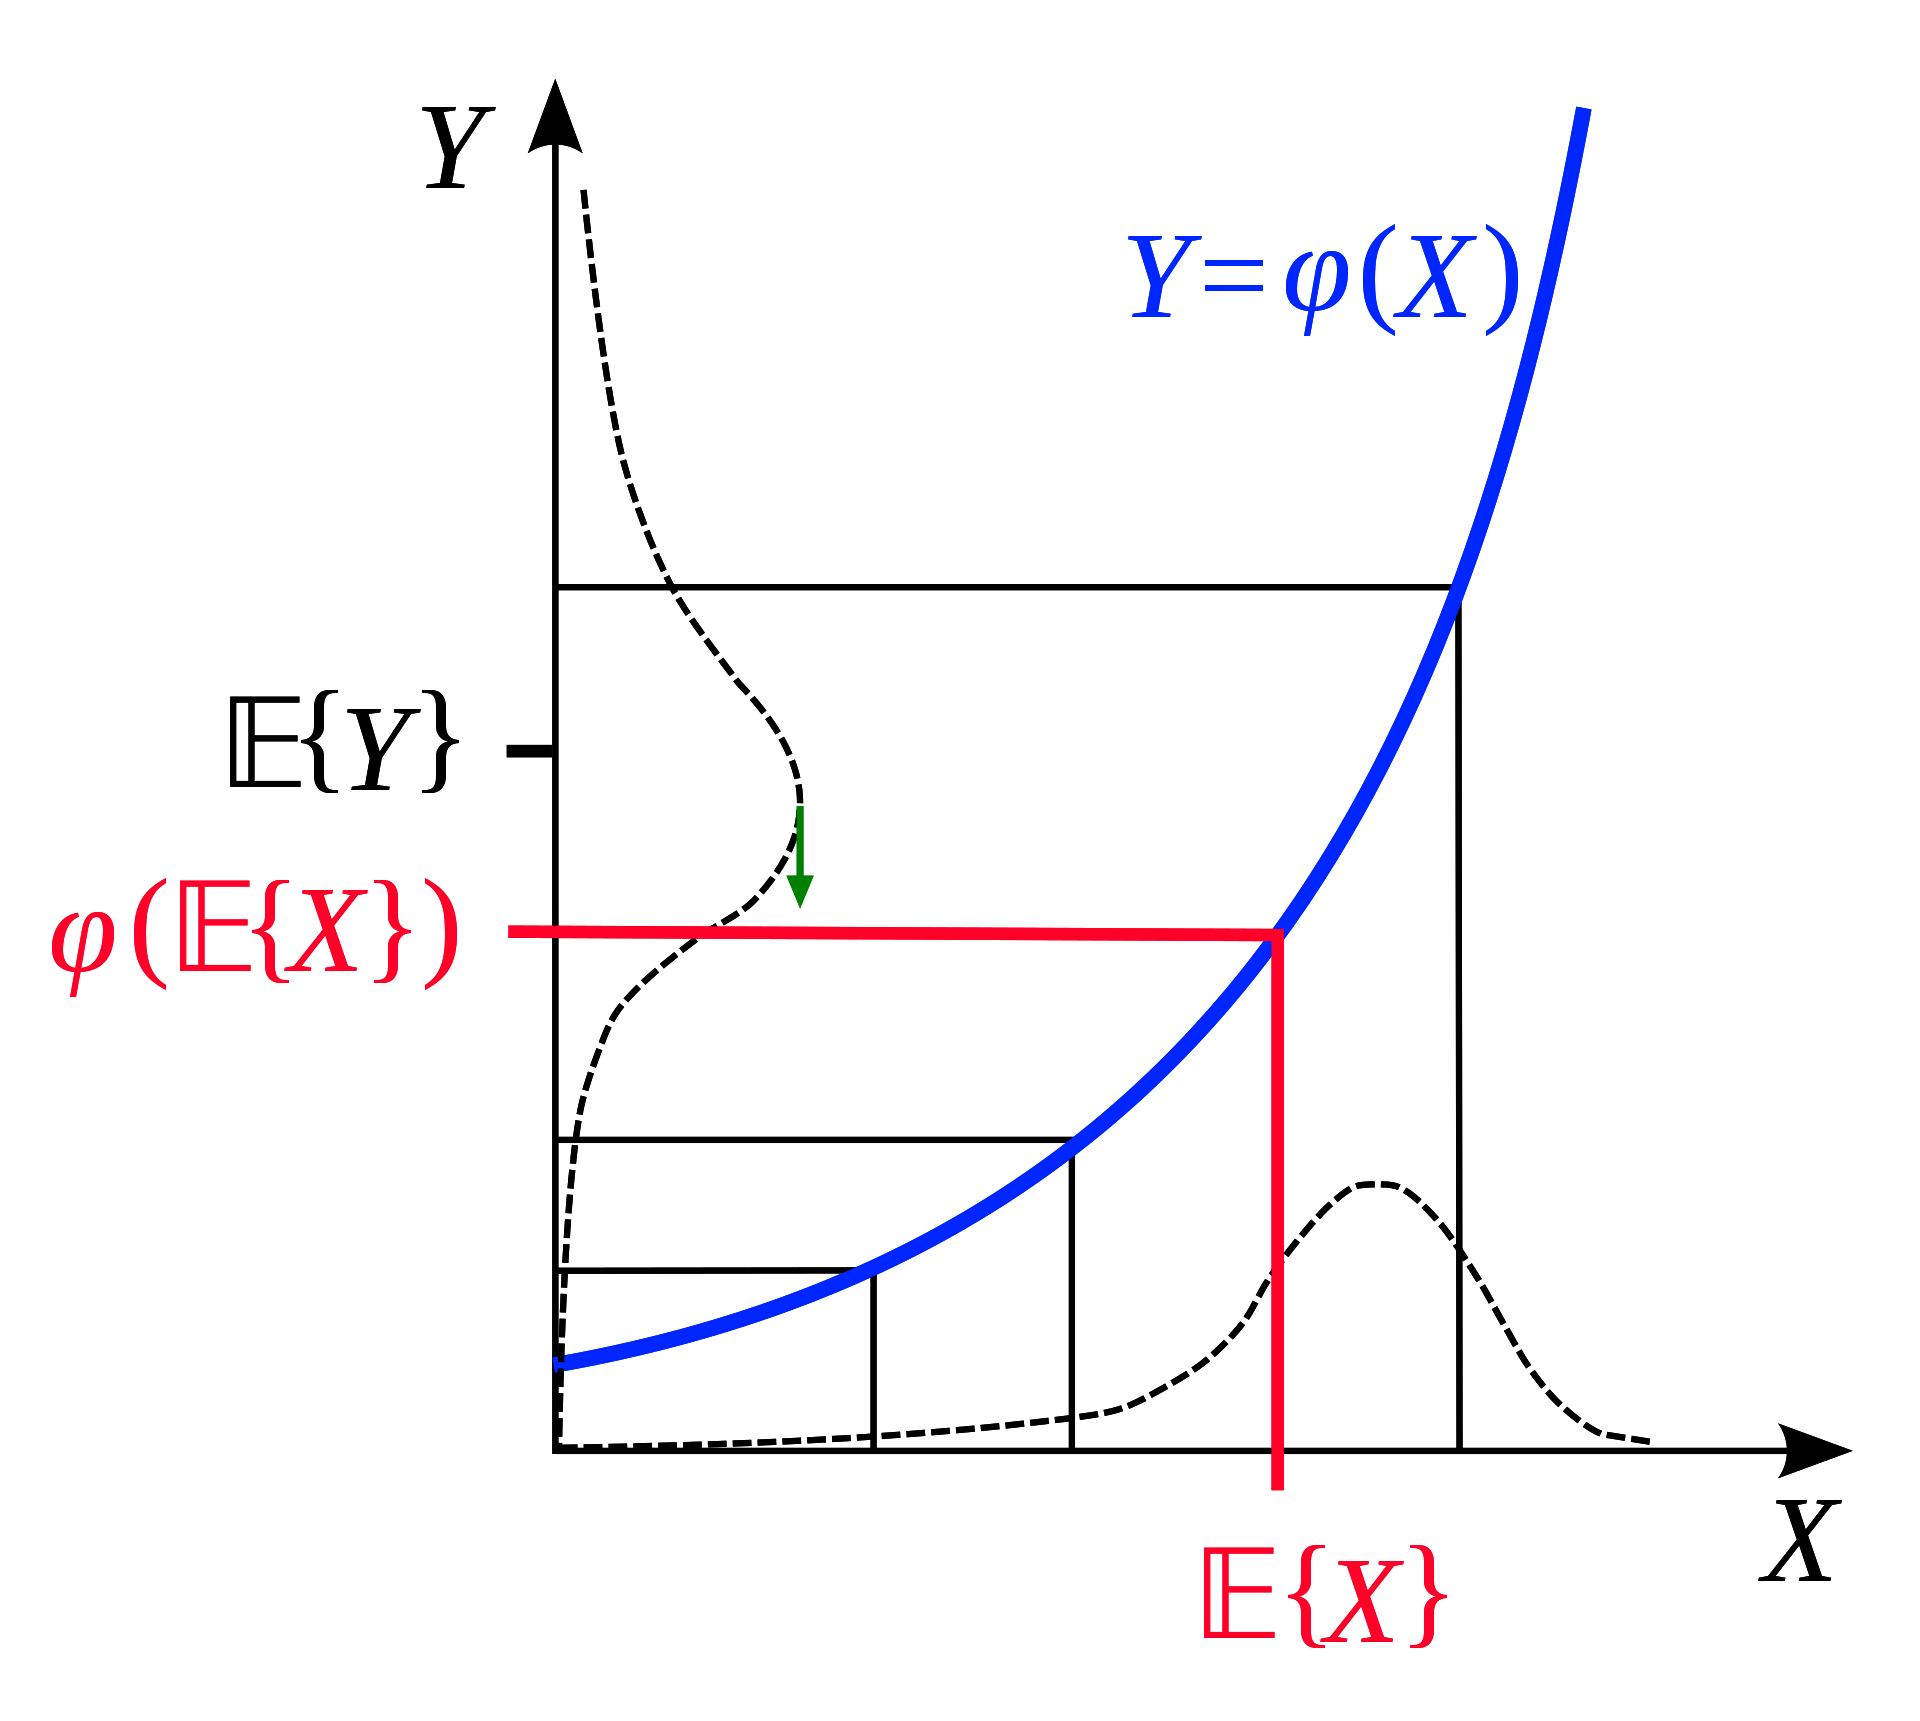
\includegraphics[width=0.9\textwidth]{resources/jensen.png}
\end{center}
\end{column}
\end{columns}



\end{frame}

\begin{frame}{More Technical Details}
Define $Y$ as the ratio of the density at $\theta$ to the density at the true value $\theta_0$ both evaluated at $Z$
\begin{align*}
Y = \frac{f_Z(Z;\theta)}{f_Z(Z;\theta_0)}
\end{align*}
\vspace{-0.5cm}
\begin{itemize}
\item Let $g(a) = -\ln(a)$ so that $g'(a) = \frac{-1}{a}$ and $g''(a) =\frac{1}{a^2}$.
\item Then by \alert{Jensen's Inequality} $\mathbb{E}[- \ln Y] \geq - \ln \mathbb{E}[Y]$.
\item This gives us
\begin{align*}
\mathbb { E }_z \left[ - \ln \left( \frac { f _ { Z } ( Z ; \theta ) } { f _ { Z } \left( Z ; \theta _ { 0 } \right) } \right) \right] \geq - \ln \left( \mathbb { E }_z \left[ \frac { f _ { Z } ( Z ; \theta ) } { f _ { Z } \left( Z ; \theta _ { 0 } \right) } \right] \right)
\end{align*}
\item The RHS is
\begin{align*}
\mathbb { E }_z \left[ \frac { f _ { Z } ( Z ; \theta ) } { f _ { Z } \left( Z ; \theta _ { 0 } \right) } \right] = \int \frac { f _ { Z } ( z ; \theta ) } { f _ { Z } \left( z ; \theta _ { 0 } \right) } \cdot f _ { Z } \left( z ; \theta _ { 0 } \right) d z = \int f _ { Z } ( z ; \theta ) d z = 1
\end{align*}
\end{itemize}
\end{frame}


\begin{frame}{More Technical Details}
Because $\log(1)=0$ this implies:
\begin{align*}
\mathbb { E }_z \left[ - \ln \left( \frac { f _ { Z } ( Z ; \theta ) } { f _ { Z } \left( Z ; \theta _ { 0 } \right) } \right) \right] \geq 0
\end{align*}
Therefore 
\begin{align*}
- \mathbb { E } \left[ \ln f _ { Z } ( Z ; \theta ) \right] &+ \mathbb { E } \left[ \ln f _ { Z } \left( Z ; \theta _ { 0 } \right) \right] \geq 0\\
\mathbb { E } \left[ \ln f _ { Z } \left( Z ; \theta _ { 0 } \right) \right] &\geq \mathbb { E } \left[ \ln f _ { Z } ( Z ; \theta ) \right]
\end{align*}
\begin{itemize}
\item We maximize the expected value of the log likelihood at the true value of $\theta$!
\item Helpful to work with $\mathbb{E}[\log f(z; \theta)]$ sometimes.
\end{itemize}
\end{frame}


\begin{frame}{Information Matrix Equality}
We can relate the \alert{Fisher Information} to the Hessian of the log-likelihood
\begin{align*}
\mathcal { I } \left( \theta _ { 0 } \right) = - \mathbb { E } \left[ \frac { \partial ^ { 2 } \ln f } { \partial \theta \partial \theta ^ { \prime } } \left( z ; \theta _ { 0 } \right) \right] 
= \mathbb { E } \left[ \frac { \partial \ln f } { \partial \theta } \left( z ; \theta _ { 0 } \right) \times \frac { \partial \ln f } { \partial \theta  } \left( z ; \theta _ { 0 } \right)' \right]
\end{align*}
\begin{itemize}
    \item This is sometimes known as the \alert{outer product of scores}.
    \item This matrix is \alert{positive semi-definite} (positive definite under identification)
    \item Recall that $ \mathbb { E } \left[ \frac { \partial \ln f } { \partial \theta } \left( z ; \theta _ { 0 } \right) \right] = 0$ at the true $\theta_0$ (and the sample mean score is $0$ at $\widehat{\theta}_{MLE}$)
\end{itemize}
\end{frame}


\begin{frame}{Proof}
\begin{align*}
1 = \int _ { z } f _ { Z } ( z ; \theta ) d z \Rightarrow 0 = \frac { \partial } { \partial \theta } \int _ { z } f _ { Z } ( z ; \theta ) d z
\end{align*}
With some regularity conditions
\begin{align*}
0 = \int _ { z } \frac { \partial f _ { Z } } { \partial \theta } ( z ; \theta ) d z = \underbrace{\int _ { z } \frac { \partial \ln f _ { Z } } { \partial \theta } ( z ; \theta ) \cdot f _ { Z } ( z ; \theta ) d z}_{\mathbb { E }_{\theta} \left[ \frac { \partial \ln f _ { Z } } { \partial \theta } \left( Z ; \theta \right) \right]}
\end{align*}

\begin{itemize}
    \item At $\theta=\theta_0$: the score has mean zero, which is the population version of the FOC.
    \item Can get information identity with another set of derivatives.
    \end{itemize}
\end{frame}


\begin{frame}{The Cram\'er--Rao Bound}
We can relate the \alert{Fisher Information} to the Hessian of the log-likelihood
\begin{align*}
\mathcal { I } ( \theta ) = - \mathbb { E } \left[ \frac { \partial ^ { 2 } \ln f } { \partial \theta \partial \theta ^ { \prime } } ( Z | \theta ) \right]
\end{align*}
It turns out this provides a bound on the variance of any \alert{unbiased} estimator from $N$ observations:
\begin{align*}
\operatorname { Var } ( \hat { \theta } ) \geq \left[ N \, \mathcal { I } \left( \theta _ { 0 } \right) \right] ^ { - 1 }
\end{align*}
Since $\sqrt{N}(\widehat{\theta}_{MLE}-\theta_0) \stackrel{d}{\longrightarrow} \mathcal{N}(0,\mathcal{I}(\theta_0)^{-1})$, the MLE attains the bound asymptotically: it is \alert{asymptotically efficient} (if the model is correctly specified).
\end{frame}

\begin{frame}{MLE: Discussion}
Tradeoffs
\begin{itemize}
\item How does this compare to GM Theorem?
\item If MLE is the most efficient estimator, why ever use something else?
\end{itemize}
\end{frame}



\begin{frame}{Examples}
We are going to practice writing down the:
\begin{itemize}
\item Likelihood $L(\theta)= \Pr(z_1,\ldots,z_n ; \theta) = \prod_{i=1}^N f(z_i ; \theta)$.
\item log likelihood $\ell(\theta)= \sum_{i=1}^N \ln f(z_i ; \theta) = \sum_{i=1}^N \ell_i(z_i ; \theta)$.
\item Scores $\mathcal{S}_i(z_i, \theta) =\frac{\partial \ln f(z_i ; \theta)}{\partial \theta}=\frac{\partial \ell_i(z_i ; \theta)}{\partial \theta}$.
\item Hessian contribution $\mathcal{H}_i(z_i, \theta) =\frac{\partial^2 \ell_i(z_i ; \theta)}{\partial \theta \partial \theta'}$.
\item Information Matrix $\mathcal{I}(\theta) = \mathbb{E}_z[-\mathcal{H}_i(z_i,\theta)]=\mathbb{E}_z[\mathcal{S}_i(z_i,\theta) \mathcal{S}_i(z_i,\theta)^T]$
\item Variance of any unbiased estimator $\geq [N\,\mathcal{I}(\theta)]^{-1} $ (Cram\'er--Rao Lower Bound).
\end{itemize}

\end{frame}


\begin{frame}{Exponential Example}
\begin{itemize}
\item Suppose we have data that are exponentially distributed $Y_i \sim \text{Exp}(\lambda)$. The goal is to estimate the parameter $\lambda$ via MLE and $f(y_i | \lambda) = \lambda e^{-\lambda y_i}$ so that $\E[y_i]=\frac{1}{\lambda}$.
\item Sometimes we want to parameterize the rate  $\lambda_i = x_i' \beta$ with covariates (this requires $x_i'\beta>0$; $\lambda_i=\exp(x_i'\beta)$ is the usual choice).
\item Example: Time until next customer arrives varies with time of day, day of week, etc. Time until default might depend on credit score, debt-to-income, market conditions, etc.
\end{itemize}
\end{frame}



\begin{frame}{Exponential Regression Example (Careful: two parameterizations here!)}
\begin{align*}
\text{For } y_i > 0, \quad f _ { y \mid x} ( y_i \mid x_i , \beta  ) =  (x_i \, \beta)e^{ - (x_i \beta )\, y_i }\, \quad  \text{ so that } \E[y_i] = \frac{1}{x_i\, \beta}
\end{align*}
With log likelihood
\begin{align*}
\ell( \beta ) = \sum _ { i = 1 } ^ { N } \ln f _ { y \mid x } \left( y _ { i } \mid x _ { i } , \beta \right) = \sum _ { i = 1 } ^ { N } \log(x _ { i } ^ { \prime }\, \beta) - \left( x _ { i } ^ { \prime }\, \beta \right)\, y _ { i } 
\end{align*}
And Score, Hessian, and Information Matrix:
\begin{align*}
\frac{\partial\, \ell_i}{\partial\, \beta} = \mathcal { S }_i ( y_i, x_i , \beta ) &=  x_i ^ { \prime } \left( \frac{1}{x_i\, \beta} - y_i \right)\\
\frac{\partial^2\, \ell_i}{\partial\, \beta \partial\, \beta'} = \mathcal { H }_i ( y_i , x_i , \beta ) &= - \frac{x_i'\, x_i}{(x_i'\, \beta)^2}\\
\mathcal { I } \left( \beta _ { 0 } \right) &= \sum_i \frac{x_i' x_i}{(x_i\, \beta)^2}
\end{align*}
\end{frame}


\section*{Computing Maximum Likelihood Estimators}

\begin{frame}{Newton's Method for Root Finding}
Consider the Taylor series for $f(x)$ approximated around $x_0$:
\begin{align*}
f(x) \approx f(x_0) + f'(x_0) \cdot (x-x_0) + \tfrac{1}{2} f''(x_0) \cdot (x-x_0)^2 + O\big((x-x_0)^3\big)
\end{align*}
Suppose we wanted to find a \alert{root} of the equation where $f(x^{*})=0$ and solve for $x$:
\begin{align*}
0 &= f(x_0) + f'(x_0) \cdot (x-x_0) \\
x_1 &= x_0-\frac{f(x_0)}{f'(x_0)} 
\end{align*}
This gives us an \alert{iterative} scheme to find $x^{*}$:
\begin{enumerate}
\item Start with some $x_0$. Calculate $f(x_k),f'(x_k)$
\item Update using $x_{k+1} = x_k - \frac{f(x_k)}{f'(x_k)} $
\item Stop when $|x_{k+1}-x_{k}| < \epsilon_{tol}$.
\end{enumerate}
\end{frame}

\begin{frame}{Newton-Raphson for Optimization}
We can re-write \alert{optimization} as \alert{root finding}:
\begin{itemize}
\item We want to know $\hat{\theta} = \arg \max_{\theta} \ell(\theta)$.
\item Construct the FOCs $\frac{\partial \ell}{\partial \theta}=0$ and find the zeros.
\item How? using Newton's method! Set $f(\theta) = \frac{\partial \ell}{\partial \theta}$
\end{itemize}
\begin{align*}
\theta_{k+1} &= \theta_k -  \left[ \frac{\partial^2 \ell}{\partial \theta^2}(\theta_k) \right]^{-1} \cdot \frac{\partial \ell}{\partial \theta}(\theta_k)
\end{align*}
The SOC (for a maximum) is that $ \frac{\partial^2 \ell}{\partial \theta^2} <0$. Ideally at all $\theta_k$.\\
This is all for a \alert{single variable} but the \alert{multivariate} version is basically the same.
\end{frame}


\begin{frame}{Newton's Method: Multivariate}
Start with the objective $Q(\theta) = - \ell(\theta)$:
\begin{itemize}
\item Approximate $Q(\theta)$ around some initial guess $\theta^{(0)}$ with a quadratic function
\item Minimize the quadratic function (because that is easy) call that $\theta^{(1)}$
\item Update the approximation and repeat.
\begin{align*}
\theta_{k+1} = \theta_k - \left[ \frac{\partial^2 Q}{\partial \theta \partial \theta'}(\theta_k) \right]^{-1}\frac{\partial Q}{\partial \theta}(\theta_k)
\end{align*}
\item The equivalent SOC is that the {Hessian Matrix} of $Q$ is \alert{positive definite}  (ideally at all $\theta$).
\item In that case $Q$ is \alert{strictly convex}, so any stationary point is its \alert{unique global minimum} (the maximum of $\ell$) and is easy to find.
\end{itemize}
\end{frame}


\begin{frame}{Newton's Method}
We can generalize to Quasi-Newton methods:
\begin{align*}
\theta_{k+1} = \theta_k -  \lambda_k \underbrace{\left[ \frac{\partial^2 Q}{\partial \theta \partial \theta'} \right]^{-1}}_{A_k} \frac{\partial Q}{\partial \theta}(\theta_k)
\end{align*}
Two Choices:
\begin{itemize}
\item Step length $\lambda_k$
\item Step direction $d_k=A_k \frac{\partial Q}{\partial \theta}(\theta_k)$
\item Often rescale the direction to be unit length $\frac{d_k}{\norm{d_k}}$.
\item If we use $A_k$ as the true Hessian and $\lambda_k=1$ this is a \alert{full Newton step}.
\end{itemize}
\end{frame}

\begin{frame}{Newton's Method: Alternatives}
Choices for $A_k$
\begin{itemize}
\item $A_k= I_{k}$ (Identity) is known as \alert{gradient descent} or \alert{steepest descent}
\item BHHH. Specific to MLE. Exploits the \alert{Fisher Information}.
\begin{align*}
A _ { k } 
&= \left[ \sum _ { i = 1 } ^ { N } \frac { \partial \ln f } { \partial \theta } \left( z_i, \theta _ { k } \right) \frac { \partial \ln f } { \partial \theta ^ { \prime } } \left( z_i, \theta _ { k } \right) \right] ^ { - 1 }, \quad \text{because}\\
\frac{1}{N}\sum_{i=1}^N \frac { \partial \ln f } { \partial \theta } \frac { \partial \ln f } { \partial \theta ^ { \prime } } &\stackrel{p}{\longrightarrow} \mathbb { E } \left[ \frac { \partial \ln f } { \partial \theta } \left( Z , \theta _0 \right) \frac { \partial \ln f } { \partial \theta ^ { \prime } } \left( Z , \theta _0 \right) \right] = - \mathbb { E } \left[ \frac { \partial ^ { 2 } \ln f } { \partial \theta \partial \theta ^ { \prime } } \left( Z , \theta _0 \right) \right]
\end{align*}
\item Quasi-Newton alternatives \alert{BFGS} (the usual default), \alert{SR1}, and \alert{DFP} start from an initial estimate of the Hessian matrix and then cheaply update $A_k$.
\item Usually computing (and inverting) the Hessian is the costly step.
\item Non invertible Hessians are bad news.
\end{itemize}
\end{frame}


\section*{Thanks!}

\end{document}